\subsubsection{Training-set size (H4)}

To test whether the gap shrinks as more data become available, we trained all models on 10\%, 25\%, 50\%, 75\%, and 100\% of the training split, drawn at random for each seed with stratification, and evaluated them on the same test split as before. The training budget stayed fixed (learning rate 0.05, 200 epochs), and the preprocessing was refitted on each subset. Fig.~\ref{fig:h4} shows the learning curves and Table~\ref{tab:h4} the paired difference between the VQC and the MLP.

\begin{figure*}[t]
\centering
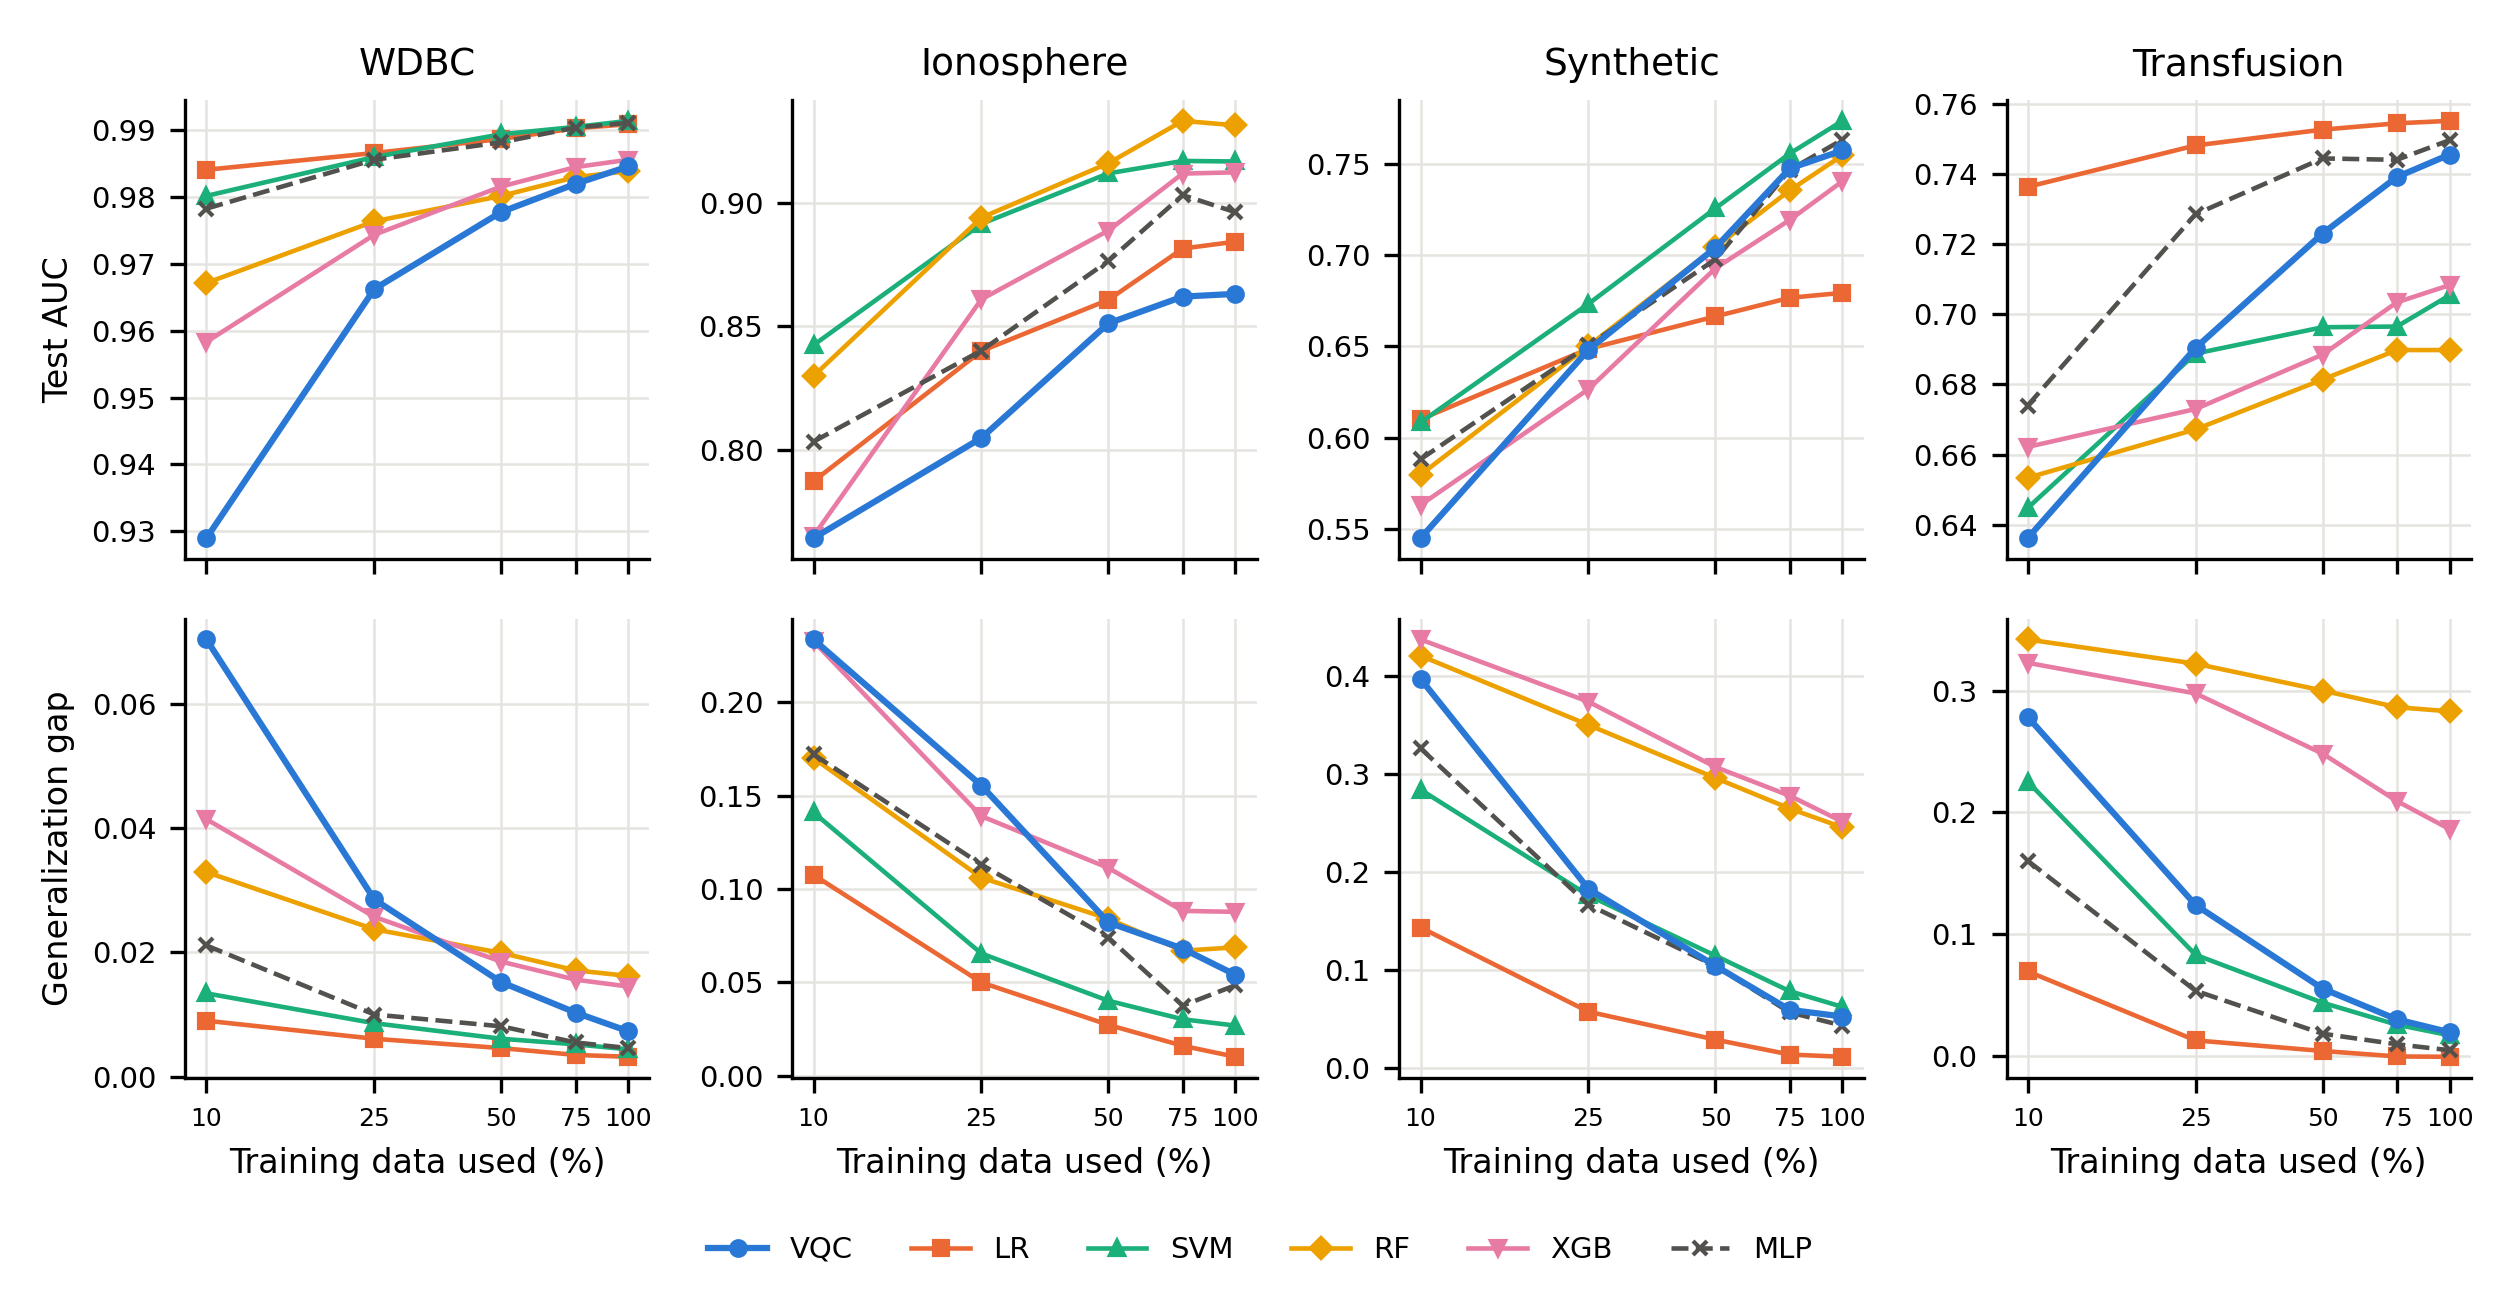
\includegraphics[width=0.9\textwidth]{fig_h4.png}
\caption{Test AUC (top) and generalization gap (bottom) as a function of the percentage of the training split used, for the VQC and the classical models, averaged over 30 seeds.}
\label{fig:h4}
\end{figure*}

\textit{The gap shrinks with more data, and more for the VQC.} The gap of the VQC decreased from 0.070 to 0.007 on WDBC, from 0.234 to 0.054 on Ionosphere, from 0.397 to 0.052 on the synthetic data, and from 0.278 to 0.019 on Blood Transfusion between 10\% and 100\% of the data, and its test AUC increased by 0.056, 0.099, 0.213, and 0.109. The MLP showed the same trend with smaller changes (gap decreases of 0.016, 0.124, 0.283, and 0.156; test AUC increases of 0.013, 0.093, 0.175, and 0.076). Logistic regression had the smallest gap at every size on all four datasets, whereas the Random Forest and XGBoost still had gaps between 0.014 and 0.283 with the full training split.

\textit{At small sizes, the VQC generalized worse than the MLP.} With 10\% of the data, the gap of the VQC was larger than that of the MLP on all four datasets ($+0.049$ on WDBC, $+0.061$ on Ionosphere, $+0.071$ on the synthetic data, and $+0.118$ on Blood Transfusion, with intervals above zero), and its test AUC was lower ($-0.049$, $-0.039$, $-0.043$, and $-0.038$; the interval on Blood Transfusion ended at $-0.000$). The difference in gap shrank with more data, but not in the same way on every dataset (Table~\ref{tab:h4}). On WDBC and Blood Transfusion it decreased steadily (to $+0.003$ and $+0.015$ with the full split). On the synthetic data it was close to zero from 50\% of the data on ($0.000$ at 50\% and $+0.009$ with the full split, with intervals including zero), and on Ionosphere it was not monotonic ($+0.008$ at 50\%, $+0.030$ at 75\%, and $+0.006$ with the full split). With the full split, the test AUC of the VQC was still lower than that of the MLP on WDBC ($-0.006$) and on Ionosphere ($-0.033$), and similar on the other two datasets.

\begin{table*}[t]
\centering
\caption{Paired difference between the VQC and the MLP when trained on a fraction of the training split (columns, percentage of the training data), mean over 30 seeds. At 10\% the training sets had 24 to 52 samples, and at 100\% they had 245 to 523. A dagger marks a 95\% bootstrap interval that excludes zero (no multiple-comparison correction).}
\label{tab:h4}
\footnotesize
\setlength{\tabcolsep}{3pt}
\begin{tabular}{llccccc}
\hline
Dataset & Metric & 10\% & 25\% & 50\% & 75\% & 100\% \\
\hline
WDBC & $\Delta$ test AUC & $-$0.049$^{\dagger}$ & $-$0.019$^{\dagger}$ & $-$0.010$^{\dagger}$ & $-$0.008$^{\dagger}$ & $-$0.006$^{\dagger}$ \\
 & $\Delta$ gap & 0.049$^{\dagger}$ & 0.019$^{\dagger}$ & 0.007$^{\dagger}$ & 0.005$^{\dagger}$ & 0.003$^{\dagger}$ \\
Ionosphere & $\Delta$ test AUC & $-$0.039$^{\dagger}$ & $-$0.035$^{\dagger}$ & $-$0.025$^{\dagger}$ & $-$0.041$^{\dagger}$ & $-$0.033$^{\dagger}$ \\
 & $\Delta$ gap & 0.061$^{\dagger}$ & 0.042$^{\dagger}$ & 0.008 & 0.030$^{\dagger}$ & 0.006 \\
Synthetic & $\Delta$ test AUC & $-$0.043$^{\dagger}$ & $-$0.002 & 0.006 & 0.001 & $-$0.006 \\
 & $\Delta$ gap & 0.071$^{\dagger}$ & 0.016 & 0.000 & 0.003 & 0.009 \\
Transfusion & $\Delta$ test AUC & $-$0.038 & $-$0.038$^{\dagger}$ & $-$0.021$^{\dagger}$ & $-$0.005 & $-$0.004 \\
 & $\Delta$ gap & 0.118$^{\dagger}$ & 0.071$^{\dagger}$ & 0.037$^{\dagger}$ & 0.020$^{\dagger}$ & 0.015$^{\dagger}$ \\
\hline
\end{tabular}
\end{table*}
